\chapter{\textbf{Traitement d'images}}
    \section{Introduction}
    Les systèmes ANPR sont essentiellement des technologies axées sur le traitement d’images numériques. Les images sont dans une certaine mesure à un système ANPR ce que la matière première est pour l’industrie. Elles passent par de plusieurs transformations et d’opérations afin d'extraire une information qui est le numéro d’immatriculation sous format textuel. Ce chapitre permet donc de présenter ces différentes transformations et opérations. Mais avant d’y arriver commençons par exposer les généralités sur les images numériques.

    \section{Généralités sur les images numériques}
    \subsection{Qu'est-ce qu'une image numérique ?}
    Une image numérique est toute image (dessin, icône, photographie, etc) acquise, créée, traitée ou stockée sous forme binaire (suite de 0 et de 1) :
    \begin{itemize}
        \item[•]\textbf{Acquise} par des dispositifs comme les scanners, les appareils photo ou caméscopes numériques, les cartes d’acquisition vidéo (qui numérisent directement une source comme la télévision).
        \item[•]\textbf{Créée} directement par des programmes informatiques, via la souris, les tablettes graphiques ou par la modélisation 3D (ce que l’on appelle par abus de langage les « images de synthèse »).
        \item[•]\textbf{Traitée} grâce à des outils informatiques. Il est facile de la modifier en taille, en couleur, d’ajouter ou supprimer des éléments, d’appliquer des filtres variés, etc.
        \item[•]\textbf{Stockée} sur un support informatique (disquette, disque dur, CD-ROM(Compact Disk Read Only Memory), etc ) \cite{wikiImage}
    \end{itemize}
    \subsection{Représentation de l'image}
    Selon la manière dont les images sont représentées pour être visualisées sur les écrans des ordinateurs, on distingue deux grandes classes d’images numériques à savoir les images matricielles et les images vectorielles.
    \begin{itemize}
        \item[•]\textbf{Les images matricielles}: encore appelées images bitmap, elles sont représentées à travers des matrices de points à plusieurs dimensions. Dans le cas de deux dimensions spatiales (largeur, hauteur), on parle d’\textbf{images 2D} et les points sont appelés \textbf{pixels (Picture Element)}. C’est le type le plus répandu. Si une image 2D possède en plus un composant temporel \textbf{(image 2D + t)}, on parle dans ce cas d’\textbf{animation}. Si par contre l’image possède trois dimensions spatiales (largeur, hauteur, profondeur), on parle d’\textbf{image 3D} ou volume et les points sont appelés \textbf{voxels (Volume Element)}.
        \item[•]\textbf{Les images vectorielles}: les données d'une image vectorielle sont représentées par des formes géométriques (cercle, rectangle, ...) qui sont décrites mathématiquement. Elles possèdent l’avantage contrairement aux images vectorielles d’occuper moins d’espace mémoire et la flexibilité dans le redimensionnement sans perte d’informations.
    \end{itemize}
    \begin{figure}[H]
        \centering
        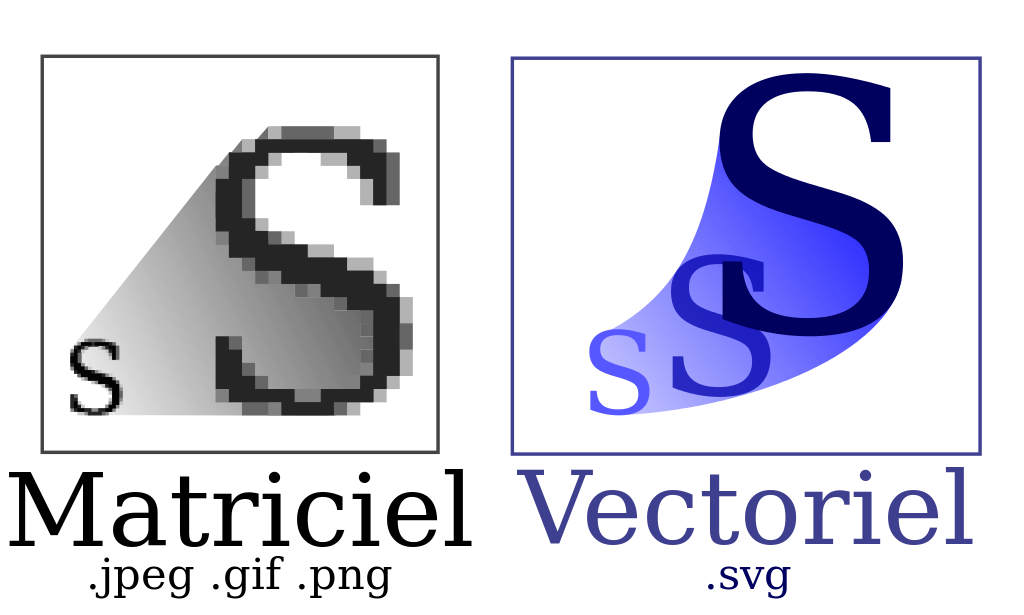
\includegraphics[scale=0.3]{matricielleVSvectorielle}
        \caption{Différence entre image matricielle et image vectorielle}
    \end{figure}
    Dans la famille des images matricielles, on distingue trois types d’images:
    \begin{itemize}
        \item[•]\textbf{Les images binaires}: elles sont uniquement en noir et blanc. La matrice de représentation contient uniquement des 0 et 1.
        \item[•]\textbf{Les images en niveaux de gris}: la matrice de représentation contient des valeurs entières entre 0 et 255 qui correspondent au niveau d’intensité lumineuse.
        \item[•]\textbf{Les images de couleur}: elles sont régulièrement obtenues par une synthèse additive des trois couleurs fondamentales :rouge, vert, bleu (RVB ou RGB en anglais). La matrice de représentation est constituée dans ce cas de trois matrices: pour chaque couleur, une matrice dont chaque cellule donne l’intensité lumineuse de la couleur correspondante.
    \end{itemize}
    \begin{figure}[H]
        \begin{subfigure}{0.3\textwidth}
            \centering
            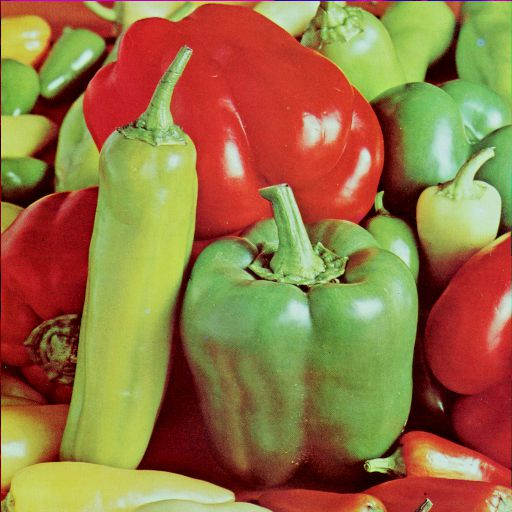
\includegraphics[width=\textwidth]{food}
            \caption{Image de couleur}
        \end{subfigure}
        \hfill
        \begin{subfigure}{0.3\textwidth}
            \centering
            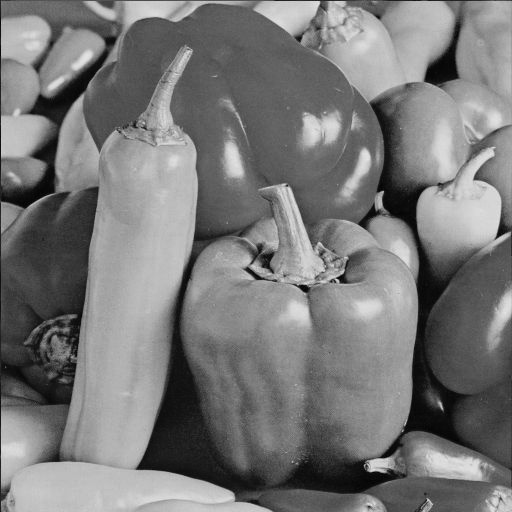
\includegraphics[width=\textwidth]{food_gray}
            \caption{Image en niveau de gris}
        \end{subfigure}
        \hfill
        \begin{subfigure}{0.3\textwidth}
            \centering
            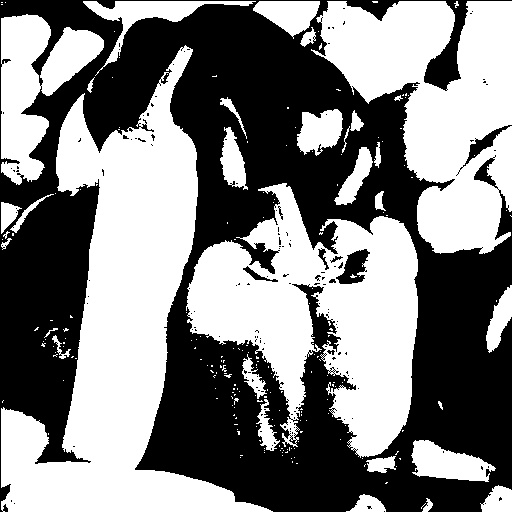
\includegraphics[width=\textwidth]{food_binary}
            \caption{Image binaire}
        \end{subfigure}
        \caption{Exemples de types d'images matricielles}
    \end{figure}
	Dans le cadre de notre projet, nous travaillons exclusivement avec les images matricielles 2D. Donc pour la suite, lorsqu’on parle d’image, il s'agit d’une image matricielle 2D sauf s’il est mentionné le contraire. 
    \subsection{Caractéristiques d'une image numérique}
    Une image a trois caractéristiques principales:
    \begin{itemize}
        \item[•]\textbf{Les dimensions}: elles représentent la largeur et la hauteur de l’image généralement exprimées en pixels.
        \item[•]\textbf{La définition}: c’est le nombre de pixels constituant une image. Elle est obtenue en multipliant le nombre de pixels sur la largeur par le nombre de pixels sur la hauteur.
        \item[•]\textbf{La résolution}: c’est le nombre de pixels que l’on retrouve sur une unité de longueur. Elle s’exprime généralement en ppp (point par pouce) ou encore en anglais dpi (dot per inch).  Plus la résolution est importante, plus les points sont petits et nombreux, plus l’image est fine.
    \end{itemize}

    \subsection{Formats des images numériques}
    Le format d’une image est la représentation informatique de cette image. Il donne les informations nécessaires sur la manière dont l’image a été codée et éventuellement des moyens de la décoder et de la manipuler. Il existe plusieurs formats qui plus ou moins adaptés pour certains cas d’utilisation:

    \begin{itemize}
        \item[•]\textbf{Format \acrfull{gif}}: ce format permet la transparence et la compression des images animées en plusieurs images séquentielles à l’intérieur du même fichier.
        Il est utilisé pour des logos, des icônes, des boutons et autres éléments de pages web. Le format d’image GIF n’atteigne au maximum que 256 couleurs, il n’est donc pas du tout adapté aux photos et à l’impression.
        \item[•]\textbf{Format \acrfull{tiff}}: un des formats le plus couramment utilisé pour stocker des images, des photographies. Il est couramment utilisé dans les environnements professionnels et pour l’impression commerciale. Il est considéré comme étant le format le plus fiable pour des impressions de haute qualité comme pour le textile, les tissus.
        \item[•]\textbf{Format \acrfull{jpg}}: c’est le format le plus adéquat pour administrer les photos et les publier. C'est l'un des formats les plus utilisés sur le net (les navigateurs l’affichent correctement) et dans les mails. Les appareils photo numériques compacts prennent également les photos au format JPG.
        \item[•]\textbf{Format \acrfull{png}}: un des formats le plus couramment utilisé. Créé pour remplacer le GIF. Performant, il réunit presque tous les avantages du JPEG et du GIF et permet les fonds transparents. \cite{akacemMaster}
        \item[•]\textbf{Format \acrfull{svg}}: contrairement aux précédents formats, SVG est un format d’images vectorielles. Il est conçu pour décrire un ensemble de graphiques vectoriels en utilisant le langage \acrshort{xml}. Cette conception permet aux images sous ce type de format d’être agrandies à l’infini sans impact sur la qualité. On utilise généralement ce format pour échanger des graphiques sur internet ou dans des logiciels de dessin assisté par ordinateur(DAO) pour représenter les objets.    
    \end{itemize}
    \section{Opérateurs de traitement d'images}
À l’instar des opérateurs mathématiques, les opérateurs de traitement d’images prennent en entrée une image et un ensemble d’informations relatives à cette image, effectuent des modifications sur ces entrées et retournent une nouvelle image ou un ensemble d’informations relatives aux données d’entrée. Ces opérateurs sont nombreux. Mais nous allons en citer quelques-unes.
    \subsection{Opérations morpho-mathématiques}
Les opérations morpho-mathématiques sont des opérations qui traitent des images en fonction de formes. Elles appliquent un élément structurant à une image d'entrée, créant une image de sortie de même taille. Dans une opération morphologique, la valeur de chaque pixel de l'image de sortie est basée sur une comparaison du pixel correspondant de l'image d'entrée avec ses voisins. Elles peuvent être utilisées pour supprimer les bruits sur une image. Les principales opérations morphologiques sont:
    \begin{itemize}
        \item[•]\textbf{La dilatation}: la valeur du pixel de sortie est la valeur maximale de tous les pixels du voisinage. Dans une image binaire, un pixel est défini sur 1 si l'un des pixels voisins a la valeur 1. La dilatation morphologique rend les objets plus visibles et comble les petits trous dans les objets.
        \begin{figure}[H]
            \centering
            
\includegraphics[scale=0.7]{dilatation}
            \caption{Dilatation}
        \end{figure}  
       
        \item[•]\textbf{L'érosion}: la valeur du pixel de sortie est la valeur minimale de tous les pixels du voisinage. Dans une image binaire, un pixel est défini sur 0 si l'un des pixels voisins a la valeur 0. L'érosion morphologique supprime les îles et les petits objets de sorte que seuls les objets substantifs restent. 
        \begin{figure}[H]
            \centering
            
\includegraphics[scale=0.7]{erosion}
            \caption{Érosion}
        \end{figure}  
        \item[•]\textbf{L'ouverture}: l'opération d'ouverture érode une image puis dilate l'image érodée, en utilisant le même élément structurant pour les deux opérations. L'ouverture morphologique est utile pour supprimer les petits objets d'une image tout en préservant la forme et la taille des objets plus gros dans l'image. 
            \begin{figure}[H]
                \centering
                
\includegraphics[scale=0.5]{opening}
                \caption{Ouverture}
            \end{figure} 
        \item[•]\textbf{La fermeture}: l'opération de fermeture dilate une image puis érode l'image dilatée, en utilisant le même élément structurant pour les deux opérations. La fermeture morphologique est utile pour combler les petits trous d'une image tout en préservant la forme et la taille des objets de l'image.\cite{mathlabMorpho}
        \begin{figure}[H]
            \centering
            
\includegraphics[scale=0.5]{closing}
            \caption{Fermeture}
        \end{figure} 
    \end{itemize} 

    \subsection{Détection des contours}
    La détection de contours est une étape essentielle du processus de traitement d’images qui permet une réduction importante de la quantité d’information relative à une image, tout en préservant des informations structurelles comme les contours et les frontières des images. Elle consiste à repérer les points d'une image numérique qui correspondent à un
    changement brutal de l'intensité lumineuse. En effet, un contour se matérialise par une rupture d'intensité
    dans l'image suivant une direction donnée. Plusieurs méthodes existent pour détecter cette rupture, les unes plus ou moins complexes, les autres plus ou moins gourmandes en calcul.

    \begin{itemize}
        \item[•]\textbf{Le filtre de Prewitt}: Prewitt est l'un des premiers algorithmes de détection de contours dans le domaine du traitement d'image.
        Il s'agit d'une approximation du gradient par convolution de l'image avec des masques de convolution.
        \item[•]\textbf{Le filtre de Sobel} : le filtre de Sobel détecte séparément les bords horizontaux et verticaux sur une image en niveaux de gris. Et on peut aussi appliquer le détecteur de Sobel sur des images en couleurs en appliquant le même
        algorithme sur les différentes composantes RGB prises séparément.
        \item[•]\textbf{Le filtre de Canny} : la méthode de Canny implémente une estimation du gradient de l'image à l'aide du filtre de Sobel, suivi
        d'un seuillage par hystérésis du module de gradient. Un seuil haut et un seuil bas sont à définir.
        Tous les pixels où le module du gradient est supérieur au premier seuil sont classifiés comme appartenant
        aux contours de l'image, des contours de l'image sont ainsi formés. Les pixels ayant un module supérieur
        au seuil bas et qui sont segmentés précédents sont définis comme points de contour dans l'image binaire
        résultante.\cite{akacemMaster}
    \end{itemize}
    \begin{figure}[H]
        \begin{subfigure}{0.3\textwidth}
            \centering
            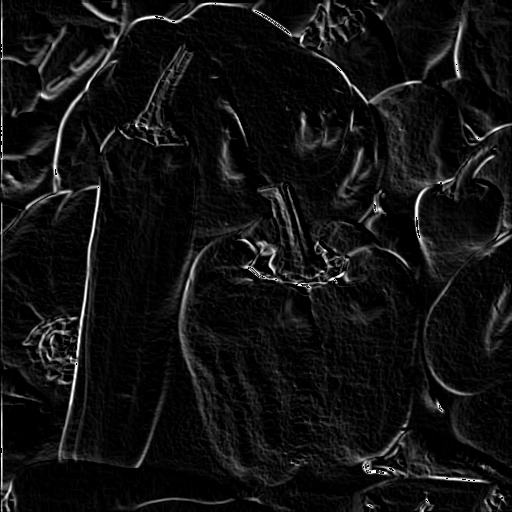
\includegraphics[width=\textwidth]{food_prewitt}
            \caption{Filtre de Prewitt}
        \end{subfigure}
        \hfill
        \begin{subfigure}{0.3\textwidth}
            \centering
            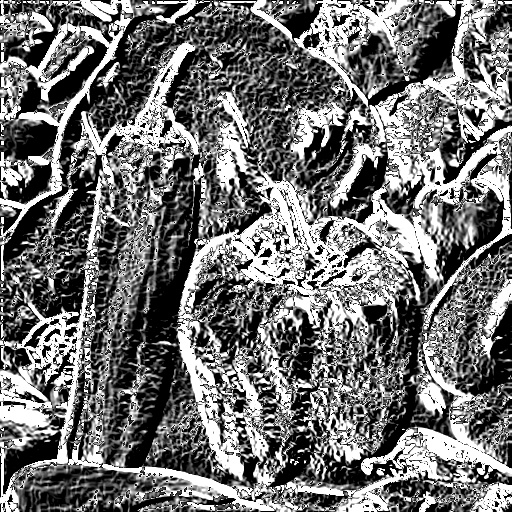
\includegraphics[width=\textwidth]{food_sobel}
            \caption{Filtre de Sobel}
        \end{subfigure}
        \hfill
        \begin{subfigure}{0.3\textwidth}
            \centering
            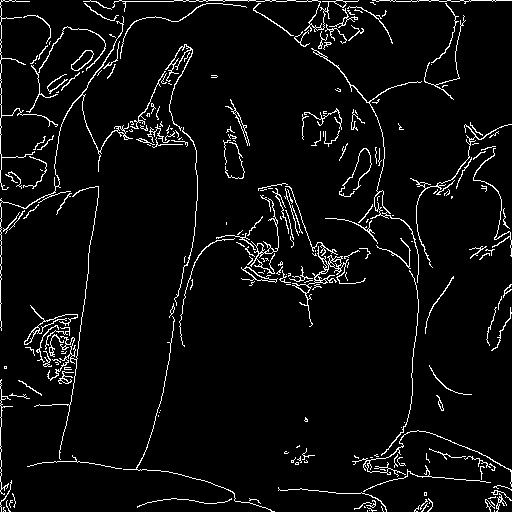
\includegraphics[width=\textwidth]{food_canny}
            \caption{Filtre de Canny}
        \end{subfigure}
        \caption{Détection des contours avec différents filtres}
    \end{figure}




    \section{Conclusion}
    La vision par ordinateur n’est possible qu’à travers une série d’algorithmes de traitement de d’images qui ont été développées depuis de très longues années. Ces algorithmes puissants permettent d’une part de modifier une image numérique  et d’autre part d'y  extraire des informations. Au cours de ce chapitre, après avoir donné quelques généralités sur les images numériques, nous avons présenté brièvement quelques méthodes qui ont été proposées pour les traiter. Par ailleurs, le traitement d’images numériques possède de nombreuses applications dont l’une qui entre dans le processus des systèmes ANPR est la reconnaissance optique de caractères. C’est l’objet du chapitre suivant. 
